% bei Standalone in documentclass noch:
% \RequirePackage{luatex85}

\documentclass[captions=tableheading, titlepage= firstiscover, parskip = half , bibliography=totoc]{scrartcl}
%paper = a5 fÃŒr andere optinen
% titlepage= firstiscover
% bibliography=totoc fÃŒr bibdateien
% parskip=half  VerÀnderung um AbsÀtze zu verbessern

\usepackage{scrhack} % nach \documentclass
\usepackage[aux]{rerunfilecheck}
\usepackage{polyglossia}
\usepackage[style=numeric, backend=biber]{biblatex} % mit [style = alphabetic oder numeric] nach polyglossia
\addbibresource{lit.bib}
\setmainlanguage{german}

\usepackage[autostyle]{csquotes}
\usepackage{amsmath} % unverzichtbare Mathe-Befehle
\usepackage{amssymb} % viele Mathe-Symbole
\usepackage{mathtools} % Erweiterungen fÃŒr amsmath
\usepackage{fontspec} % nach amssymb
% muss ins document: \usefonttheme{professionalfonts} % fÌr Beamer PrÀsentationen
\usepackage{longtable}
\usepackage{dsfont}
\usepackage[
math-style=ISO,    % \
bold-style=ISO,    % |
sans-style=italic, % | ISO-Standard folgen
nabla=upright,     % |
partial=upright,   % /
]{unicode-math} % "Does exactly what it says on the tin."
\setmathfont{Latin Modern Math}
% \setmathfont{Tex Gyre Pagella Math} % alternativ

\usepackage[
% die folgenden 3 nur einschalten bei documenten
locale=DE,
separate-uncertainty=true, % Immer Fehler mit ±
per-mode=symbol-or-fraction, % m/s im Text, sonst \frac
]{siunitx}

% alternativ:
% per-mode=reciprocal, % m s^{-1}
% output-decimal-marker=., % . statt , fÃŒr Dezimalzahlen

\usepackage[
version=4,
math-greek=default,
text-greek=default,
]{mhchem}

\usepackage[section, below]{placeins}
\usepackage{caption} % Captions schöner machen
\usepackage{graphicx}
\usepackage{grffile}
\usepackage{subcaption}

% \usepackage{showframe} Wenn man die Ramen sehen will

\usepackage{float}
\floatplacement{figure}{htbp}
\floatplacement{table}{htbp}

\usepackage{mathtools}

\usepackage{booktabs}

 \usepackage{microtype}
 \usepackage{xfrac}

 \usepackage{expl3}
 \usepackage{xparse}

 % \ExplSyntaxOn
 % \NewDocumentComman \I {}  %Befehl\I definieren, keine Argumente
 % {
 %    \symup{i}              %Ergebnis von \I
 % }
 % \ExplSyntaxOff

 \usepackage{pdflscape}
 \usepackage{mleftright}

 % Mit dem mathtools-Befehl \DeclarePairedDelimiter können Befehle erzeugen werden,
 % die Symbole um AusdrÃŒcke setzen.
 % \DeclarePairedDelimiter{\abs}{\lvert}{\rvert}
 % \DeclarePairedDelimiter{\norm}{\lVert}{\rVert}
 % in Mathe:
 %\abs{x} \abs*{\frac{1}{x}}
 %\norm{\symbf{y}}

 % FÃŒr Physik IV und Quantenmechanik
 \DeclarePairedDelimiter{\bra}{\langle}{\rvert}
 \DeclarePairedDelimiter{\ket}{\lvert}{\rangle}
 % <name> <#arguments> <left> <right> <body>
 \DeclarePairedDelimiterX{\braket}[2]{\langle}{\rangle}{
 #1 \delimsize| #2
 }

\setlength{\delimitershortfall}{-1sp}

 \usepackage{tikz}
 \usepackage{tikz-feynman}

 \usepackage{csvsimple}
 % Tabellen mit \csvautobooktabular{"file"}
 % muss in table umgebung gesetzt werden


% \multicolumn{#Spalten}{Ausrichtung}{Inhalt}

\usepackage{hyperref}
\usepackage{bookmark}
\usepackage[shortcuts]{extdash} %nach hyperref, bookmark

\newcommand{\ua}[1]{_\symup{#1}}
\newcommand{\su}[1]{\symup{#1}}

\begin{document}
\begin{titlepage}
  \begin{flushleft}
 Durchführung: 17.10.2018\\
 Abgabe: 24.10.2018\\
  \end{flushleft}


%\HRule\\[1,0cm]

 \begin{center}


\textsc{\LARGE Praktikumsprotokoll V46}\\[1.5cm]
\textsc{\huge Faraday-Effekt an Halbleitern} \\[5,5cm]

Carolin Harkort\footnotemark[1], \\
Jacqueline Schlingmann\footnotemark[2] \\[1,0cm]



 \end{center}
%\HRule

 \vfill

 \footnotetext[1]{\href{mailto:carolin.harkort@tu-dortmund.de}{carolin.harkort@tu-dortmund.de}}
 \footnotetext[2]{\href{mailto:jacqueline.schlingmann@tu-dortmund.de}{jacqueline.schlingmann@tu-dortmund.de}}
\end{titlepage}


  % bei Standalone in documentclass noch:
% \RequirePackage{luatex85}

\documentclass[captions=tableheading, titlepage= firstiscover, parskip = half , bibliography=totoc]{scrartcl}
%paper = a5 fÃŒr andere optinen
% titlepage= firstiscover
% bibliography=totoc fÃŒr bibdateien
% parskip=half  VerÀnderung um AbsÀtze zu verbessern

\usepackage{scrhack} % nach \documentclass
\usepackage[aux]{rerunfilecheck}
\usepackage{polyglossia}
\usepackage[style=numeric, backend=biber]{biblatex} % mit [style = alphabetic oder numeric] nach polyglossia
\addbibresource{lit.bib}
\setmainlanguage{german}

\usepackage[autostyle]{csquotes}
\usepackage{amsmath} % unverzichtbare Mathe-Befehle
\usepackage{amssymb} % viele Mathe-Symbole
\usepackage{mathtools} % Erweiterungen fÃŒr amsmath
\usepackage{fontspec} % nach amssymb
% muss ins document: \usefonttheme{professionalfonts} % fÌr Beamer PrÀsentationen
\usepackage{longtable}
\usepackage{dsfont}
\usepackage[
math-style=ISO,    % \
bold-style=ISO,    % |
sans-style=italic, % | ISO-Standard folgen
nabla=upright,     % |
partial=upright,   % /
]{unicode-math} % "Does exactly what it says on the tin."
\setmathfont{Latin Modern Math}
% \setmathfont{Tex Gyre Pagella Math} % alternativ

\usepackage[
% die folgenden 3 nur einschalten bei documenten
locale=DE,
separate-uncertainty=true, % Immer Fehler mit ±
per-mode=symbol-or-fraction, % m/s im Text, sonst \frac
]{siunitx}

% alternativ:
% per-mode=reciprocal, % m s^{-1}
% output-decimal-marker=., % . statt , fÃŒr Dezimalzahlen

\usepackage[
version=4,
math-greek=default,
text-greek=default,
]{mhchem}

\usepackage[section, below]{placeins}
\usepackage{caption} % Captions schöner machen
\usepackage{graphicx}
\usepackage{grffile}
\usepackage{subcaption}

% \usepackage{showframe} Wenn man die Ramen sehen will

\usepackage{float}
\floatplacement{figure}{htbp}
\floatplacement{table}{htbp}

\usepackage{mathtools}

\usepackage{booktabs}

 \usepackage{microtype}
 \usepackage{xfrac}

 \usepackage{expl3}
 \usepackage{xparse}

 % \ExplSyntaxOn
 % \NewDocumentComman \I {}  %Befehl\I definieren, keine Argumente
 % {
 %    \symup{i}              %Ergebnis von \I
 % }
 % \ExplSyntaxOff

 \usepackage{pdflscape}
 \usepackage{mleftright}

 % Mit dem mathtools-Befehl \DeclarePairedDelimiter können Befehle erzeugen werden,
 % die Symbole um AusdrÃŒcke setzen.
 % \DeclarePairedDelimiter{\abs}{\lvert}{\rvert}
 % \DeclarePairedDelimiter{\norm}{\lVert}{\rVert}
 % in Mathe:
 %\abs{x} \abs*{\frac{1}{x}}
 %\norm{\symbf{y}}

 % FÃŒr Physik IV und Quantenmechanik
 \DeclarePairedDelimiter{\bra}{\langle}{\rvert}
 \DeclarePairedDelimiter{\ket}{\lvert}{\rangle}
 % <name> <#arguments> <left> <right> <body>
 \DeclarePairedDelimiterX{\braket}[2]{\langle}{\rangle}{
 #1 \delimsize| #2
 }

\setlength{\delimitershortfall}{-1sp}

 \usepackage{tikz}
 \usepackage{tikz-feynman}

 \usepackage{csvsimple}
 % Tabellen mit \csvautobooktabular{"file"}
 % muss in table umgebung gesetzt werden


% \multicolumn{#Spalten}{Ausrichtung}{Inhalt}

\usepackage{hyperref}
\usepackage{bookmark}
\usepackage[shortcuts]{extdash} %nach hyperref, bookmark

\newcommand{\ua}[1]{_\symup{#1}}
\newcommand{\su}[1]{\symup{#1}}

\begin{document}
\section{Zielsetzung}
Ziel dieses Versuchs ist es die Streuung von $\su{\alpha}$-Teilchen an einer Goldfolie zu bestimmen.
Dafür wird der differentielle Wirkungsquerschnitt der Streuung und die Abhängigkeit der Kernladungszahl Z
des Targetmaterials untersucht. \newline
Aus der Streuung kann zusätzlich durch die Energieverlustmessung der $\su{\alpha}$-Teilchen
auch die Foliendicke bestimmt werden.
\section{Theorie}
Beim Durchlauf von positiv geladenen $\su{\alpha}$-Teilchen durch Materie kann es zu
zwei unterschiedlichen Wechselwirkungen kommen. Die erste Wechselwirkung findet mit negaitv geladenen Hüllenelektron
statt und die zweite mit dem positiven Atomkern.
\newline
Bei der Wechselwirkung zwischen $\su{\alpha}$-Teilchen und dem Hüllenelektronen kommt es durch
Anregungs- und Ionisationsprozesse zur Energieabgabe.
Es wird angenommen, dass es aufgrund der größeren Masse der $\su{\alpha}$-Teilchen gegenüber
der Elektronenmasse zu keiner Ablenkung der $\su{\alpha}$-Teilchen kommt.
\newline
Die Bethe-Bloch-Gleichung beschreibt den Energieverlust
\begin{equation*}
    -\frac{dE}{dx} = -\frac{4\pi e^4z^2NZ}{m_0v^2(4\pi \epsilon_0)^2} \ln \frac{2m_0v^2}{I}
\end{equation*}
der $\su{\alpha}$-Teilchen beim Durchgang durch die Materie.
Hierbei gibt N die Atomdichte, $\su{m_0}$ die Ruheenergie des Hüllenelektrons, Z die Kernladungszahl und I die mittlere Ionisationsenergie
des Targetmaterials an.

Bei der Streuung der $\su{\alpha}$-Teilchen am Atomkern kommt es durch die Coulombkraft zu
einer Richtungsänderung um den Streuwinkel $\su{\Theta}$. Es wird nach der 1. Born'schen Näherung davon
ausgegangen, dass die Mehrfachstreuung der $\su{\alpha}$-Teilchen vernachlässigt werden kann.
\newline
Dieser Streuwinkel lässt sich mit der Rutherford-Streuformel berechnen
\begin{equation*}
    \frac{d\sigma}{d\Omega}(\Uptheta) = \frac{1}{(4\pi \epsilon_0)^2} \Big(\frac{zZe^2}{4E_{\alpha}}\Big)^2 \frac{1}{\sin^4\frac{\Uptheta}{2}}.
\end{equation*}
Der differentielle Wirkungsquerschnitt $\frac{d\sigma}{d\Omega}$ beschreibt gerade die Intensitätsverteilung
der gestreuten $\su{\alpha}$-Teilchen in den Raumwinkel $\su{\Uptheta}$.
\section{Versuchsaufbau}
Der Versuchsaufbau ist in Abbildung \ref{fig:aufbau} dargestellt.
\begin{figure}
  \centering
  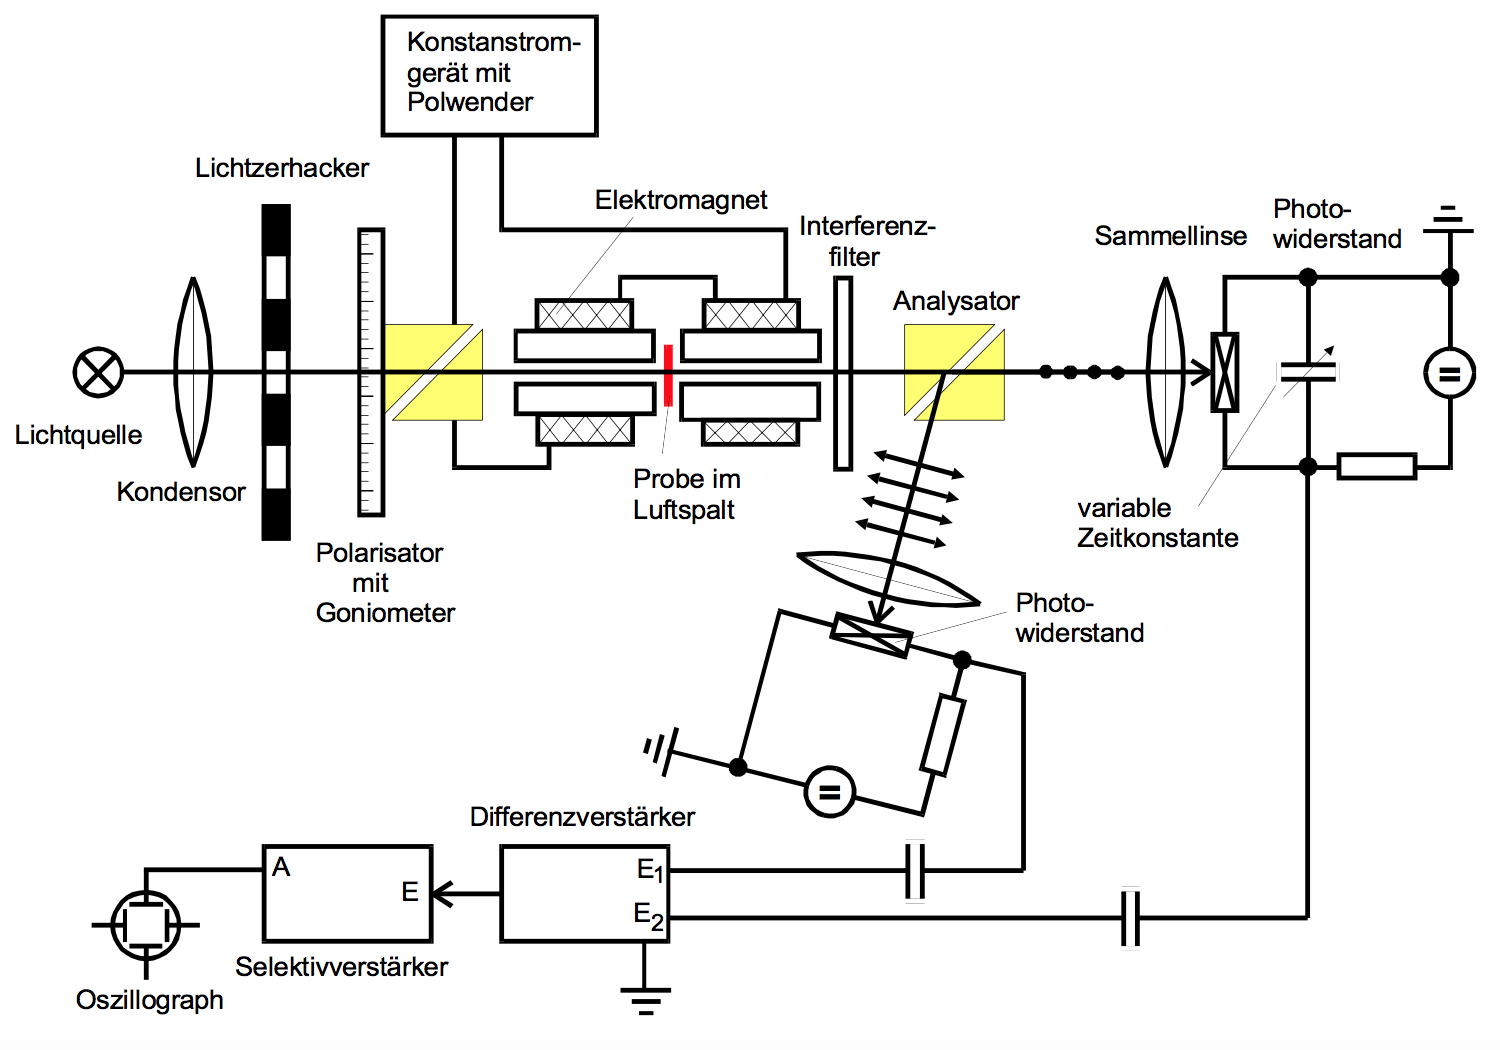
\includegraphics[width = 12 cm]{pictures/aufbau.png}
  \caption{Darstellung des Versuchsaufbaus}
  \label{fig:aufbau}
\end{figure}
\newline
Der Versuch findet im Vakuum statt, da die $\su{\alpha}$-Strahlung in Luft nur eine sehr geringe
Reichweite hat. Als $\su{\alpha}$-Strahler dient ein $\ce{^{241}}\su{Am}$-Präparat.
Die dort austretenen Teilchen werden kollimiert, damit diese senktrecht auf die Goldfolie treffen.
An dieser Folie werden die Teilchen gestreut und von einem Surface-Barrier-Detektor detektiert.

\section{Durchführung}
Zu Beginn des Versuches wird die Apparatur über eine Vakuumspumpe evakuiert.
Um einen geraden Durchtritt der $\su{\alpha}$-Teilchen sicher zu stellen, wird der Detektor zuerst
in den Strahlengang richtig hereingestellt.
\newline
Für die Bestimmung der Foliendicke wird eine Energieverlustmessung durchgeführt.
Dabei werden die Pulshöhen der Detektorpulse in Abhängigkeit des Kammerdrucks aufgenommen.
Durch das Feindrosselventil kann der Kammerdruck langsam erhöht werden.
Zur Ermittlung der mittleren Pulshöhe wird das Oszilloskop in das Programm "Nachleuchten" gestellt,
an dem dann die Pulshöhen abgelesen werden können.\newline
Diese Messung wird einmal mit und einmal ohne Goldfolie gemacht.
\newline
Um den differentiellen Wirkungsquerschnitt einer Goldfolie zu bestimmen, wird die Zählrate in Abhängigkeit
des Streuwinkels $\su{\Uptheta}$ aufgenommen. Dafür werden unterschiedliche Winkel eingestellt.
Die Dauer der Messung wird durch den statistischen Fehler der Zählrate
$\sqrt{I}$ festgelegt, da der $\su{\alpha}$-Zerfall poissonverteilt ist.
\newline
Zur Untersuchung der Mehrfachstreuung wird die Streuung der unterschiedliche Folien gemessen. Dafür wird ein fester Winkel
eingestellt.
\newline
Die Aktivität wird außerdem ohne Folie für 120\,s gemessen.
\end{document}

  %\input{durchführung.tex}
  
  \section{Auswertung}
  \subsection{Bestimmung der maximalen Kraftflussdichte}
  Die gemessenen Werte sind relativ zum Mittelpunkt der Helmholtzspule aufgenommen.
  An diesem Punkt ist das Magnetfeld am größten.
  Die Werte sind in Tabelle \ref{tab:Bfeld} zu finden.

  \begin{table}
    \centering
    \caption{gemessene Kraftflussdichte}
    \label{tab:Bfeld}
    \begin{tabular}{c c}
      \toprule
      B(z)/ \si{\milli\tesla} & $\symup{z_{rel}}$ / \si{\centi\meter}\\
      \midrule
       68  & 14\\
       136 & 12\\
       254 & 10\\
       350 & 8 \\
       407 & 6 \\
       436 & 4 \\
       450 & 2 \\
       464 & 0 \\
       458 & -2\\
       451 & -4\\
       437 & -6\\
       404 & -8\\
       335 &-10\\
       210 &-12\\
       98  &-14\\
      \bottomrule
    \end{tabular}
  \end{table}

Um die maximale Kraftflussdichte zu ermitteln wird B(z) gegen z aufgetragen.
Dies ist in Abbildung \ref{fig:Bfeld} zu sehen.
Die lineare Regression wird mit der Formel
\begin{equation*}
 B(z) = m \cdot (z-a)^2 + n
\end{equation*}
durchgeführt.
So ergeben sich die Parameter
\begin{align*}
m &= (-2,01 \pm 0,08)\,\mathrm{\frac{mT}{cm^2}}\\
a &= (-0,62 \pm 0,16)\,\mathrm{cm}\\
n &= (481,17 \pm 8,13)\,\mathrm{mT}\\
\Rightarrow S &=(-0,62, 481,17)
\end{align*}
Somit liegt das Maximum bei
\begin{equation}
\symup{B_{max}}= (481,17\pm 8,13)\,\mathrm{mT} .
\label{eqn:bfeld}
\end{equation}
\begin{figure}
  \centering
  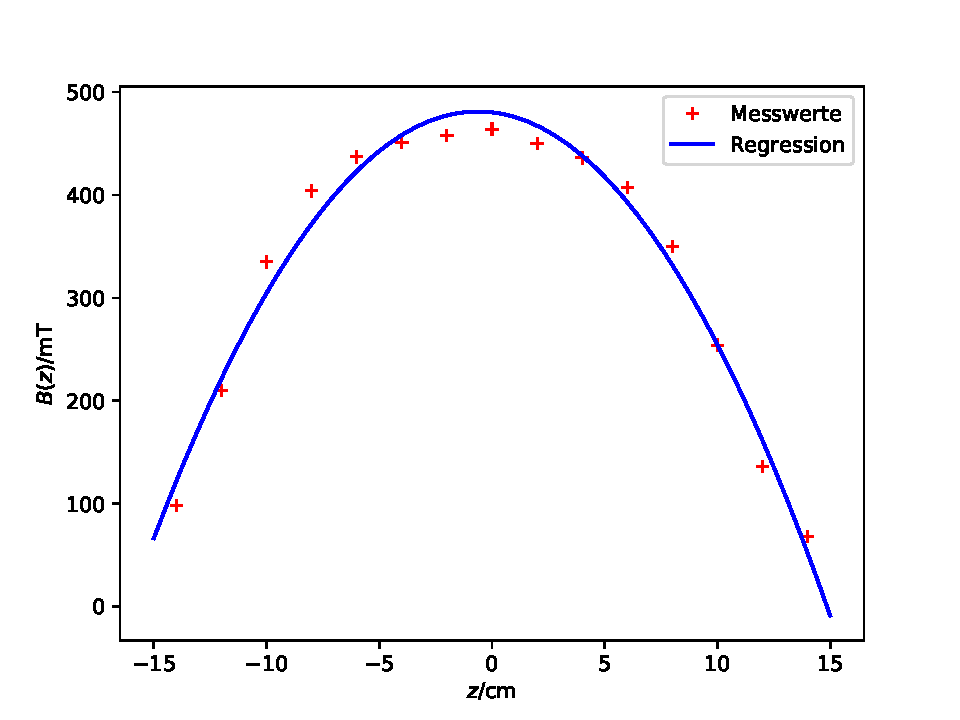
\includegraphics[width=\textwidth]{plotbfeld.pdf}
  \caption{gemessene Kraftflussdichte}
  \label{fig:Bfeld}
\end{figure}

\subsection{Messung der Faraday-Rotation}
Die Messergebnisse des n-dotierten GaAs sind in Tabelle \ref{tab:ndotiert} aufgetragen.
Die Probe hat eine Dicke von D=$1,36\,\mathrm{mm}$ und N=$1,2\cdot 10^{18}\,\mathrm{cm^3}$.

  \begin{table}
    \centering
    \caption{n-dotiertes GaAs}
    \label{tab:ndotiert}
    \begin{tabular}{c c c c c}
      \toprule
      $\lambda/ \si{\micro\meter}$ & $\theta_1 / °$ & $\theta_2 /°$ & $\theta_{\symup{reell}}/°$ &
      $\Delta\theta_{\symup{norm}}/\frac{1}{\mathrm{m}}$\\
      \midrule
       1,06  & 189 & 186 & 1,5 & 19,25 \\
       1,29  & 190 & 188 & 1,0 & 12,83  \\
       2,34  & 211 & 210 & 0,5 & 6,42  \\
       2,51  & 213 & 210 & 1,5 & 19,25 \\
       2,9   & 306 & 283 & 11,5& 147,58\\
       3,18  & 223 & 208 & 7,5 & 96,25 \\
       3,985 & 320 & 312 & 4,0 & 51,33 \\
       5,3   & 231 & 216 & 7,5 & 96,25 \\
       \bottomrule
    \end{tabular}
  \end{table}

  Die Messergebnisse der hochreinen Probe
  mit einer Dicke von $D=5,1\,\mathrm{mm}$ sind in Tabelle \ref{tab:hochrein} aufgetragen.

  \begin{table}
    \centering
    \caption{hochreines GaAs}
    \label{tab:hochrein}
    \begin{tabular}{c c c c c}
      \toprule
      $\lambda/ \si{\micro\meter}$ & $\theta_1 / °$ & $\theta_2 /°$ & $\theta_{\symup{reell}}/°$ &
      $\Delta\theta_{\symup{norm}}/\frac{1}{\mathrm{m}}$\\
      \midrule
       1,06  & 208 & 207 & 0,5 & 1,71\\
       1,29  & 200 & 198 & 1,0 & 3,42\\
       2,34  & 208 & 206 & 1,0 & 3,42\\
       2,51  & 209 & 207 & 1,0 & 3,42\\
       2,9   & 234 & 228 & 4,0 & 10,25\\
       3,18  & 238 & 220 & 9,0 & 30,74\\
       3,985 & 223 & 215 & 4,0 & 13,66\\
       5,3   & 259 & 250 & 4,5 & 15,37\\
       \bottomrule
    \end{tabular}
  \end{table}

  $\theta_{\symup{reel}}$ entspricht hierbei der halbierten Differenz von $\theta_1$ und $\theta_2$.
  $\theta_{\symup{norm}}$ ist der längennormierte Winkel.
  In Abbildung \ref{fig:b} wurde der längennormierte Winkel gegen das quadrat der Wellenlänge aufgetragen
  \begin{figure}
    \centering
    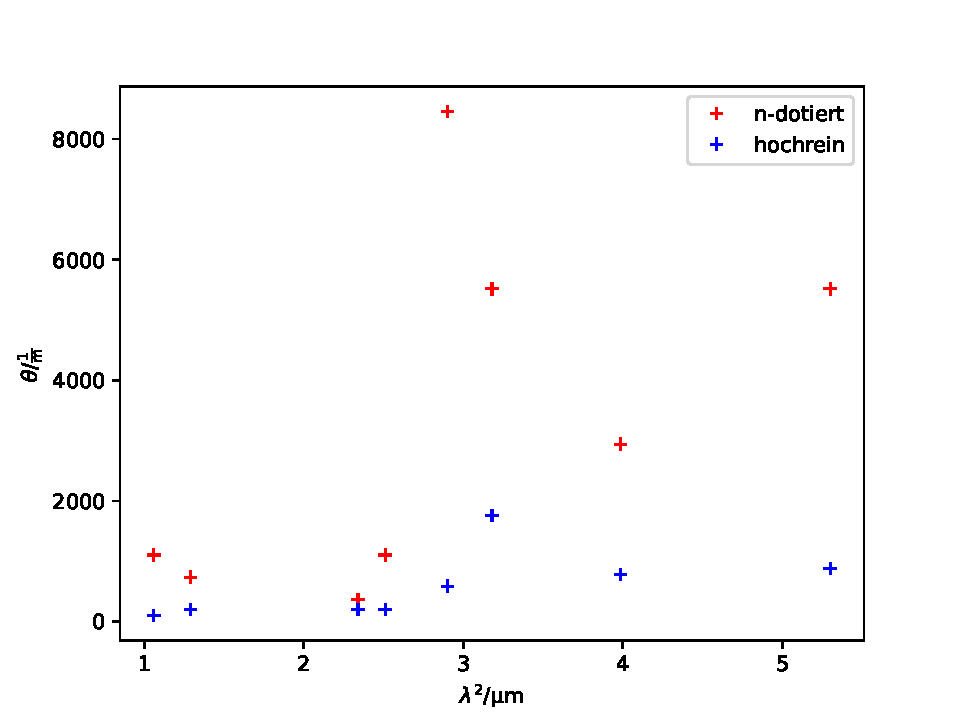
\includegraphics[width=\textwidth]{plotGaAs.pdf}
    \caption{Der Winkel gegen $\lambda ^2$ }
    \label{fig:b}
  \end{figure}

\subsection{Bestimmung der effektiven Masse}
Zur Bestimmung der effektiven Masse wird die Differenz der beiden normierten Winkel der n-dotierten
und der hochreinen Probe gebildet. Die Ergebisse sind in Tabelle \ref{tab:dif} zu finden.
Diese Winkel, aufgetragen gegen die Wellenlänge zum Quadrat, werden in Abbildung \ref{fig:dif} dargestellt.


\begin{table}[H]
  \centering
  \caption{n-dotiertes GaAs}
  \label{tab:dif}
  \begin{tabular}{c c }
    \toprule
    $\lambda/ \si{\micro\meter}$ & $\theta_{\symup{diff}} / \frac{1}{m}$ \\
    \midrule
     1,06  & 17,54\\
     1,29  & 9,42\\
     2,34  & 3,00\\
     2,51  & 15,83\\
     2,9   & 137,34\\
     3,18  & 65,51\\
     3,985 & 37,67\\
     5,3   & 80,88\\
     \bottomrule
  \end{tabular}
\end{table}
\begin{figure}[H]
  \centering
  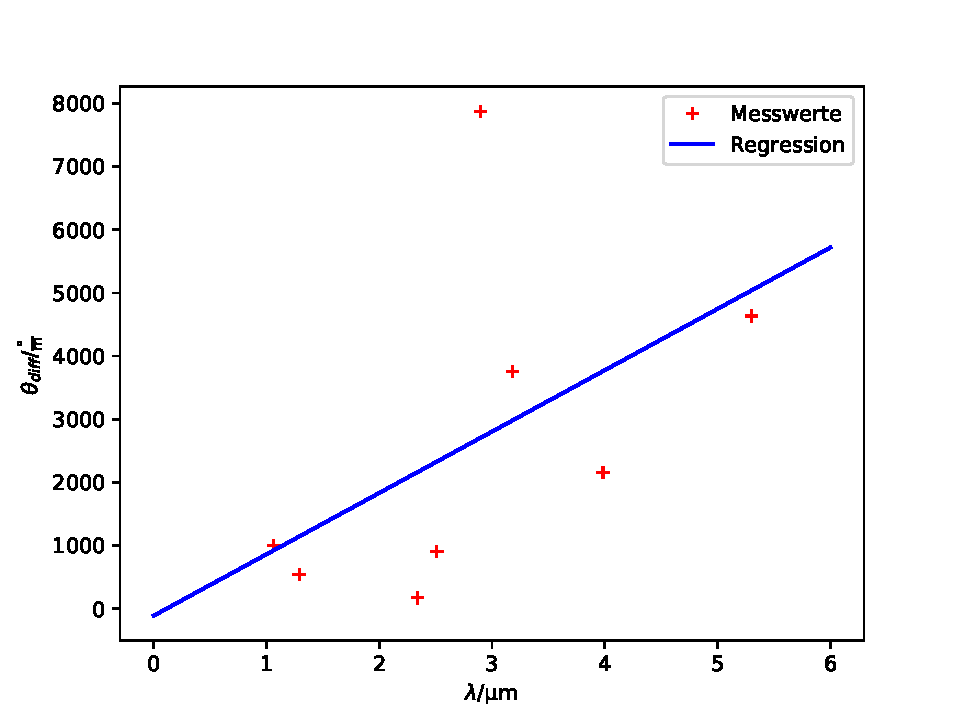
\includegraphics[width=\textwidth]{tdiff.pdf}
  \caption{Die Winkeldifferenz gegen $\lambda ^2$ }
  \label{fig:dif}
\end{figure}
Die linerare Regression wurde mit
\begin{equation*}
  \theta(\lambda^2) = a\cdot \lambda^2
\end{equation*}
durchgeführt.
Der Parameter lautet:
\begin{align*}
  a &= (23\pm24) \,\mathrm{\frac{1}{\mu m^3}}\\
\end{align*}

Mit Formel \ref{eqn:meff} ergibt sich
\begin{equation*}
a = \frac{e_0^3}{8\pi^2\epsilon_0c^3}\frac{1}{m*^2}\frac{NB}{n}
\end{equation*}
Dabei ist n der Brechungsindex und liegt bei n=3,6\cite{Brechungsindex} für eine Wellenlänge von ungefähr 886\, nm \cite{n2}.
Nach der effektiven Masse umgestellt wird die Formel zu
\begin{equation*}
  m* =\sqrt{\frac{e_0^3}{8\pi^2\epsilon_0c^3}\frac{1}{a}\frac{NB}{n}}.
\end{equation*}
Der Wert für B wird aus \ref{eqn:bfeld} übernommen und der für N liegt,
wie oben bereits erwähnt, bei N=$1,2\cdot 10^{18}\,\mathrm{cm^3}$.
Somit lautet das Ergebnis für die effektive Masse:
\begin{equation*}
  m* =(1,2\pm 0,5)\cdot10^{-32}\, \mathrm{kg}
\end{equation*}
Der Fehler berechnet sich mit
\begin{equation*}
  \Delta m* = \sqrt{\left(\frac{dm*}{dB}\cdot \Delta B\right)+\left(\frac{dm*}{da}\cdot \Delta a\right)^2}
\end{equation*}

\section{Diskussion}

Die Messung der Kraftflussdichte hat gut funktioniert.
An der Abbildung \ref{fig:Bfeld} ist zu erkennen, dass die gemessenen Werte nicht stark von der Regression abweichen.
So sind auch die Fehler der Parameter eher gering.

Die Messung der Faraday-Rotation war schwierig, da die Sinuswelle am Oszilloskop stark geflackert und geschwankt hat.
Außerdem wurde bei größeren Wellenlängen weniger Licht vom Interferenzfilter durchgelassen,
sodass nur noch ein sehr kleines Signal an den Differenzverstärker gelangen konnte.
Die Interferenzfilter waren teilweise sehr stark verschmutzt.
Hinzu kam, dass der Lichtstrahl eine Leichte Ablenkung hatte, was die Justierung stark erschwert hat.
Ein Minimum war somit Teilweise nicht wirklich zu erkennen, sodass die aufgenommenen Werte eine sehr große Fehlerbelastung haben.
Des weiteren war das Ablesen der Winkel aufgrund einer Fehlbedienung nur auf 1° genau möglich.
Das erklärt auch die Ergebnisse aus den Abbildungen \ref{fig:b} und \ref{fig:dif}.

Die Werte liegen sehr verstreut und nicht auf einer Geraden,
sodass die durch die Regression erhaltenen Größen starke Fehler aufweisen.
Der Brechungsindex ist, anders als angenommen, keine konstante Größe und somit auch eine Fehlerquelle.
Das angelegte Magnetfeld trägt ebenfalls zu den Fehlern bei, da es nicht konstant gehalten werden konnte
und Aufgrund von Überhitzung zeitweise komplett zusammen brach.
Dies führt schließlich auch dazu, dass der Fehler der berechneten effektiven Masse extrem hoch ist.
Mit dem Literaturwert $\sfrac{m*}{m_e}=0,067$ \cite{meff} und der berechneten effektiven Masse
\begin{equation*}
  \frac{m*}{m_e} = (0,013 \pm 0,005)
\end{equation*}
ergibt sich eine Abweichung von $80,60\%$.


\nocite{*}
\printbibliography
\end{document}
